\documentclass[10pt]{article}

\usepackage{fancyhdr}
\usepackage{extramarks}
\usepackage{amsmath}
\usepackage{amsthm}
\usepackage{amsfonts}
\usepackage{tikz}

\usepackage{ragged2e}
\usetikzlibrary{automata,positioning}
\usepackage{setspace}
\usepackage{etoolbox}
\usepackage{enumitem}
\usepackage{hyperref}
\hypersetup{colorlinks=true,allcolors=blue}
\usepackage{hypcap}
\usepackage{graphicx}    %for figure environment.
\usepackage{calc}
\usepackage{ifthen}
\usepackage{tikz}
\usepackage{longtable}
\usepackage{lipsum}
\usepackage{verbatim}
\usepackage{enumitem}
\setlist[enumerate]{itemsep=0mm}
\setlist[itemize]{itemsep=0mm}
\usepackage{pstricks-add}
\usepackage{pstricks}
\usepackage{rotating}
\usepackage[]{algorithm2e}


\makeatletter
\pretocmd{\@sect}{\singlespacing}{}{}
\pretocmd{\@ssect}{\singlespacing}{}{}
\apptocmd{\@sect}{\singlespacing}{}{}
\apptocmd{\@ssect}{\singlespacing}{}{}
\makeatother

%
% Basic Document Settings
%
\newcommand{\ts}{\textsuperscript}

%\begin{comment}
\topmargin=-0.45in
\evensidemargin=0in
\oddsidemargin=0in
\textwidth=6.5in
\textheight=9.0in
\headsep=0.25in
%\end{comment}

\linespread{1.1}

\pagestyle{fancy}
\lhead{\hmwkAuthorName}
\chead{\textbf{\hmwkClass : \hmwkTitle}}
\rhead{\hmwkAuthorNumber}
\lfoot{\lastxmark}
\cfoot{\thepage}

\renewcommand\headrulewidth{0.4pt}
\renewcommand\footrulewidth{0.4pt}

\setlength\parindent{0pt}

%
% Create Problem Sections
%


\setcounter{secnumdepth}{0}
\newcounter{partCounter}
\newcounter{homeworkProblemCounter}
\setcounter{homeworkProblemCounter}{1}
\nobreak\extramarks{Problem \arabic{homeworkProblemCounter}}{}\nobreak{}

%
% Homework Problem Environment
%
% This environment takes an optional argument. When given, it will adjust the
% problem counter. This is useful for when the problems given for your
% assignment aren't sequential. See the last 3 problems of this template for an
% example.
%


%
% Homework Details
%   - Title
%   - Due date
%   - Class
%   - Section/Time
%   - Instructor
%   - Author
%

\newcommand{\hmwkTitle}{Assignment 2\ \ }
\newcommand{\hmwkDueDate}{Sunday, November 12\ts{th}, 2017}
\newcommand{\hmwkClass}{CSC411}
\newcommand{\hmwkClassTime}{Section A}
\newcommand{\hmwkClassInstructor}{Steven Chuang}
\newcommand{\hmwkClassTeachingAssistant}{Natalia Mykhaylova}
\newcommand{\hmwkAuthorName}{Gokul K. Kaushik}
\newcommand{\hmwkAuthorNumber}{999878191}
\newcommand{\schoolmate}{\textsc{School-Mate }}

\newcommand\Tstrut{\rule{0pt}{2.6ex}}       % "top" strut
\newcommand\Bstrut{\rule[-0.9ex]{0pt}{0pt}} % "bottom" strut
\newcommand{\TBstrut}{\Tstrut\Bstrut} % top&bottom struts
%
% Title Page
%

\title{
    \vspace{2in}
    \textmd{\textbf{\hmwkClass:\ \hmwkTitle}}\\
    \vspace{0.1in}\small{Due\ on\ \hmwkDueDate}\\
    \vspace{3in}
    \vspace{0.1in}\large{Student Name: \textbf{\hmwkAuthorName} } \\
    \vspace{0.1in}\large{Student Number: \textbf{\hmwkAuthorNumber} } \\
}

%\author{\textbf{\hmwkAuthorName}}
%\textbf{\hmwkAuthorNumber\}
\date{}

\renewcommand{\part}[1]{\textbf{\large Part \Alph{partCounter}}\stepcounter{partCounter}\\}

%
% Various Helper Commands
%

% Useful for algorithms
\newcommand{\alg}[1]{\textsc{\bfseries \footnotesize #1}}

% For derivatives
\newcommand{\deriv}[1]{\frac{\mathrm{d}}{\mathrm{d}x} (#1)}

% For partial derivatives
\newcommand{\pderiv}[2]{\frac{\partial}{\partial #1} (#2)}

% Integral dx
\newcommand{\dx}{\mathrm{d}x}

% Alias for the Solution section header
\newcommand{\solution}{\textbf{\large Solution}}

% Probability commands: Expectation, Variance, Covariance, Bias
\newcommand{\E}{\mathrm{E}}
\newcommand{\Var}{\mathrm{Var}}
\newcommand{\Cov}{\mathrm{Cov}}
\newcommand{\Bias}{\mathrm{Bias}}
\renewcommand*\contentsname{Table of Contents}

\begin{document}
\maketitle
\pagebreak

\begin{center} \tableofcontents \end{center}
\pagebreak

\clearpage
\setcounter{page}{1}

\section{1 - Class Conditional Gaussians}
\subsection{1 - Using Bayes’ rule to derive an expression for $p(y = kx, \mu,\sigma)$}
\subsection{2 - Expression for the negative likelihood function (NLL)}
\subsection{3 - Partial Derivatives of the Likelihood}
\subsection{4 - Find the maximum likelihood estimates for $\mu$ and $\sigma$}


\section{2 - Handwritten Digit Classification}
\subsection{0 - Loading the data and Plotting the Feature Means}

The means (from 700 samples per digit) for each feature (64 features in total for an 8-by-8 pixel image) for 10 digits (digit 0 to digit 9) are plotted below: 

\begin{center}
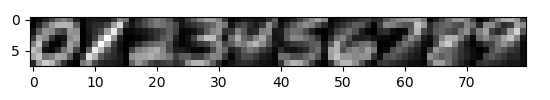
\includegraphics[scale=1]{averages.png}
\end{center}


\subsection{1 -  K-NN Classifier}
\subsubsection{Train and Test Classification Accuracy for K=1 and K=15}

\begin{center}
\begin{tabular}{lll}
                             & Accuracy                                  &                                         \\ \cline{2-3} 
\multicolumn{1}{l|}{K Value} & \multicolumn{1}{l|}{Train Classification} & \multicolumn{1}{l|}{Test Classification} \\ \hline
\multicolumn{1}{|l|}{K = 1}  & \multicolumn{1}{l|}{}                     & \multicolumn{1}{l|}{}                    \\ \hline
\multicolumn{1}{|l|}{K = 15} & \multicolumn{1}{l|}{}                     & \multicolumn{1}{l|}{}                    \\ \hline
\end{tabular}
\end{center}

\subsubsection{Tie Breaker Method}

There are cases in K-Nearest Neighbours where there isn't one most frequent neighbours (there might be two neighbours that occur equally frequently). 

Therefore, in such cases a tie breaking decision needs to be made. I have chosen to reduce the number of nearest neighbours by one - \textbf{effectively removing the last neighbour and repeating the check until a decision can be made}.

The algorithm's psuedo-code is:

\begin{algorithm}[H]
 \KwData{K Nearest Neighbours Array with a tie}
 \KwResult{Nearest Neighbours Decided}
 initialization\;
 \While{not at end of this document}{
  read current\;
  \eIf{understand}{
   go to next section\;
   current section becomes this one\;
   }{
   go back to the beginning of current section\;
  }
 }
 \caption{How to write algorithms}
\end{algorithm}
 

This method was chosen because: 
\begin{enumerate}
\item The tie remains until the \textit{most distant} neighbour from one of the most frequent neighbours is removed. This rewards the neighbour with the closest value in such cases.
\item This decision making method is intuitive to understand and easy to implement.
\end{enumerate}



\subsection{2 -  Conditional Gaussian Classifier Training}
\subsection{3 -   Naive Bayes Classifier Training}
\subsection{4 -  Model Comparison}


\pagebreak


\end{document}
